\section{心理学实验设计基本问题}

从上面的实验可以看到,\textbf{心理学实验的特点}是:

(1)影响因素多;(2)因素之间相互关联;(3)无关变量的混淆

研究者在操纵和改变自变量时候,有大量无关变量,有这么多复杂的因素需要控制,行为实验中最复杂的因素,这也是以人研究对象的实验的难点.当然我们也非常自豪地说,这是心理学家最擅长的.

我们接下来讨论什么是\textbf{实验设计}.广义的实验设计涉及的内容比较广泛,此处不予以介绍,我们看看狭义的、典型意义的实验设计要做什么.狭义的实验设计就是做好实验的计划方案、统计分析方案,就像盖房子需要一个蓝图,我们不能在盖房子前什么规划都不做就直接去盖,同样我们也不能没有计划就去进行一个实验.实验之前要做一个详细的规划,这非常重要.如果这个方案没有做好,之后便很难纠正.

\textbf{实验设计的主要目标}有三点,首先,要回答感兴趣的理论问题;其次,要获得更加丰富的信息;最后,要提高的敏感性.我们分别来看看这些目标的具体含义:

\begin{description}
	\item[1.回答感兴趣的理论问题] 
	~\
	前面已经提到了,我们感兴趣的问题是人类心理现象的规律性问题,也是对人类行为和心理现象产生的动因感兴趣.所以首先我们要建立变量之间的关系,在实验中操纵或改变一个或多个变量,并观察其对行为的影响,记录下因变量的观测指标的变化情况.
	
	但是影响某个心理或行为的因素不只有我们感兴趣的自变量那么简单,我们的想法是让不同被试仅仅在自变量上有所不同,并且这个不同是由研究者操纵的,这样结果就确定是由自变量引起的.但由于实验对象的特殊性,我们很难保重不同人在进行实验前是完全相等的,所以我们还要对那些对因变量也产生影响,但是不是为研究者所感兴趣的变量进行控制,也就是要控制无关变量,减小或控制其对因变量影响.
	
	最后,选用复杂的统计方法,在同样的数据量中得到更多有意义的信息.
	
	\item[2.更加丰富的信息]
	~\
	首先,可以选用更好的实验设计的种类,比如在多因素设计中,除了主效应,还有交互作用,而交互作用往往可以提供一些非常有用的信息.在研究中,不同因素间往往存在相互影响,忽略一个因素而研究另一个因素时,难以看到真实的结果,这就是单因素实验设计的局限.
	
	其次,可以选用丰富的因变量,这个等下举个例子说明.
	
	最后,正确选择一些复杂的统计
	
	\begin{kaobox}[frametitle=多因素实验设计的优点]
		~\
		(1)可以同时估计两个或多个实验处理的效应,可以估价实验处理之间的交互作用
		
		(2)因素实验设计可以对数据资源进行更加有效的利用,使同样数量的数据给出丰富的信息
		
		但是要注意的是,多因素实验设计的统计和解释可能会比较复杂,特别是对于一个高次的交互作用,很难解释其意义;并且,过多因素的实验设计可能设计时觉得还挺漂亮的,但是实际做出来交互作用都不显著.这提醒我们研究一个问题的时候要先深入研究该领域,,当有足够了理论支持多因素实验的交互作用显著时,多因素实验设计才可能成功.
	\end{kaobox}

	\item[3.提高实验的敏感性] 
		~\
		前面我们已经提到,处理不显著的时候,可能真的是处理效应不存在,也可能是实验设计不够敏感,我们要尽量减小后一种的可能性.不过大多时候如果处理效应不显著,我们并不能将这两者区分开来.
	
\end{description}



%记得整理一下这个实验=-= 还要自己画图嘤嘤嘤

%舒华(1996)的五张图
%字的类型和年级交互作用
\begin{marginfigure}
	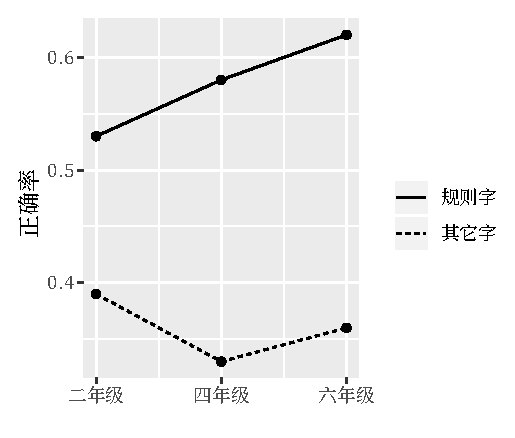
\includegraphics{shu(1996)_grade_type}
	\caption{字的类型$\times$年级}
	\labfig{shu(1996)t_g}
\end{marginfigure}

%字的类型和熟悉性交互作用
\begin{marginfigure}
	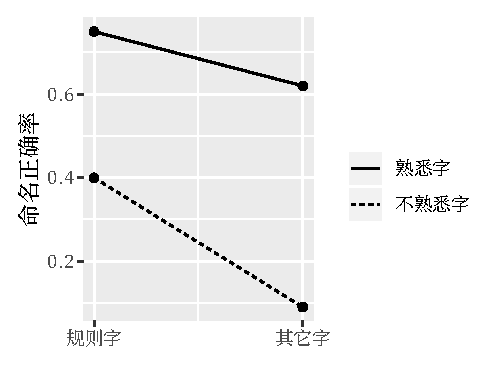
\includegraphics{shu(1996)_type_familiarity}
	\caption{字的类型$\times$熟悉性}
	\labfig{shu(1996)t_f}
\end{marginfigure}

%能力/熟悉性/类型三次交互作用图(重要! 好好解释)
\begin{marginfigure}
	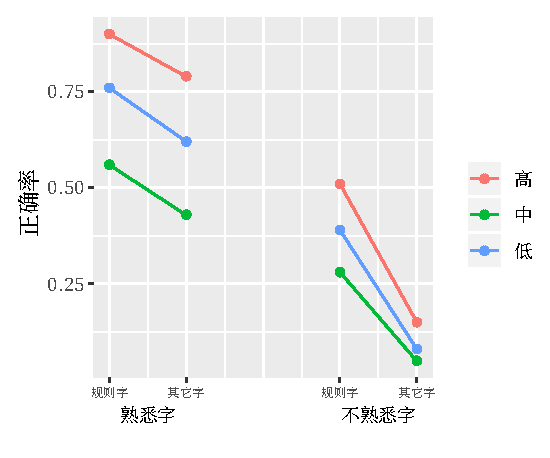
\includegraphics{shu(1996)_familiarity_type_capicity}
	\caption{能力$\times$熟悉性$\times$字的类型}
	\labfig{shu(1996)_t_f}
\end{marginfigure}

%错误分析
\begin{marginfigure}
	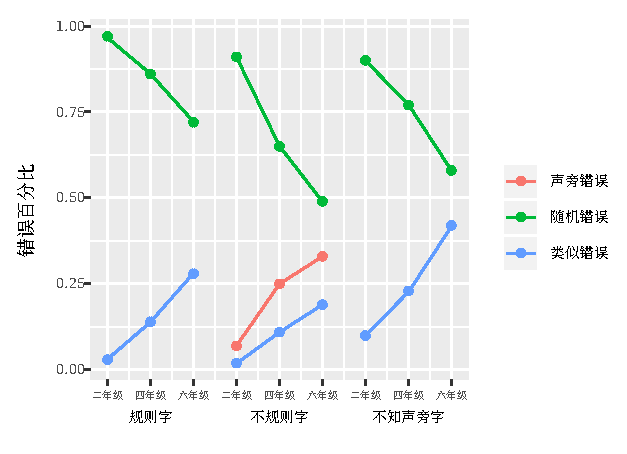
\includegraphics{shu(1996)false}
	\caption{儿童在各类字读音中犯不同类型错误占总错误的百分比}
	\labfig{shu(1996)_false}
\end{marginfigure}


%读音错误分析
\begin{marginfigure}
	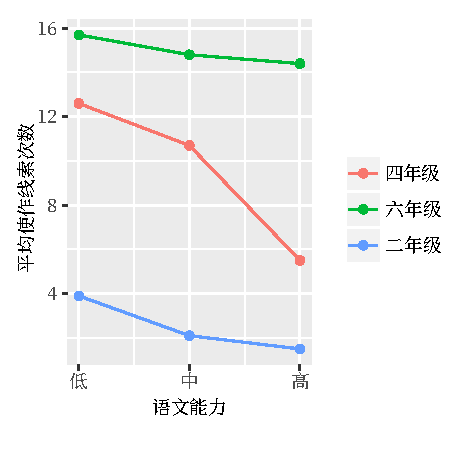
\includegraphics{shu(1996)_grade_capicity}
	\caption{儿童读音中使作线索的平均次数}
	\labfig{shu(1996)_cue}
\end{marginfigure}

舒华(1996)的一项研究中,对孩子读汉字的过程进行研究,特别是不熟悉的汉字.研究者想看到孩子读汉字能力的发展.实验中有一个非常漂亮的三次交互作用,揭示了一下有价值的信息.

这是一个3(年级)$\times$3(语文能力)$\times$2(字的熟悉性)$\times$3(字的类型)的四因素混合设计,其中字的熟悉性和字的类型是被试内变量,语文能力和年级是被试间变量.实验材料是60个单个形声字组成的卷子,所有的字都选自小学语文课本,每个年级的卷中包括30个熟悉的字和30个不有不同的字.熟悉字指学生在课本中已经学过的字,不熟悉字指学生在课本中还未学过的字,例如四年级卷子中的熟悉字选自第五、六册语文课本(三年级用书)后面的生字表,不熟悉字选自第九、十册语文课本(五年级用书)后面的生字表.每种熟悉度的字中有10个规则字,即字的声旁本身是一个儿童熟悉的汉字,且声旁的读音与字的读音相同,如“绘”;10个不规则字,即字的声旁是一个儿童熟悉的汉字,但声旁的读音与字的读音不相同,如“略”;和10个不知声旁的字,即字的声旁不是一个独立的汉字,其读音是一般人所不熟悉的,如“忱”,它的声旁“冘”的读音是“yin2”.不同熟悉度和不同类型的字的笔划数是经过匹配的,平均笔划数为10.实验是在三个自然班中集体进行的,每个学生接受相应年级的卷子,并按要求用拼音给出30个熟悉字和30个不熟悉字的读音,对写不出准确拼音的字,可以写一个与它同音的熟字代替. 

上述几个自变量比较难操作的是熟悉性.熟悉是最熟悉、全部都认识的吗?不熟悉、一定不认识的吗?这样做的话会出现天花板和地板效应,也就是熟悉的字成绩为100\%,不熟悉的字成绩为0.比较好的实验设计是,熟悉是比较熟悉,但也不是百分之百熟悉;不熟悉是相对不熟悉,也不是0.额外,上面提到,不同年级的材料间有一定的重叠这样使用的汉字数量比较少,这就减少了由汉字本身特点带来的无关变异.最后二四六年级的儿童匹配到的熟悉和不熟悉汉字的来源是:

\begin{figure}[hb]
	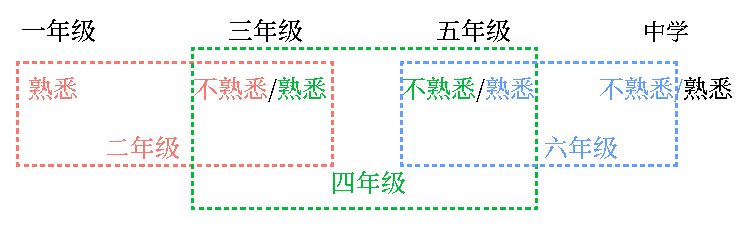
\includegraphics{shu(1996)_meterial}
	%\caption{舒华(1996)对二四六年级儿童熟悉字和不熟悉字的定义}
	\labfig{shu(1996)_meterial}
\end{figure}

年级和字的类型的交互作用显著(见\reffig{},规则字随着年龄增长,不规则字差不多,使用这个规则有一个学习过程

字的类型和熟悉性的交互作用显著,不规则的字更倾向于推理

语文能力三次交互作用显著,不熟悉的字中

对错误的分析中,三类
随机错误三类错误都下降
不规则字声旁错误增加
类似错误也是增加的
儿童对汉字的认知在发展,光读声旁很可能读错,所以在家族中找一个字

使用线索的次数,四年级有一个较大的发展

正确率由前侧,50\%正确率有较大变异

%-----------------------------------------------------------------
想要达到实验设计的目的主要通过以下三种手段:
\begin{description}
	\item[1.加大处理效应]
	有的时候增大处理效应不是一个很好的方法,因为处理效应太大了会没有意义.比如我想研究人的数学能力的发展,我选取3岁、15岁、60岁的人,可是我在实验前就已经知道60岁的人数学能力大于15岁的人大于3岁的人,这就没有研究的必要了.心理学的效应往往是日常生活中本身不太明显,以至于人们一般看不到这个现象,我们的研究就是要发现这个微弱的效应,并说明其探讨其存在意义.
	
	\item[2.减小误差]
	以方差分析为例,方差分析最后判断是否显著构成了一个$F$分布:
	$$
	F=\frac{MS_{effect}}{MS_{error}}
	$$
	
	实验的目的就是想让$F$达到显著水平,也就是$F$越大越好,上面已经否定让分子无限变大的可能性,那么分母是不是可以尽量控制让其减小呢?答案是肯定的,控制实验误差使其很小是实验设计的中心问题.
	
	\begin{kaobox}[frametitle=通过实验设计减小误差的方法]
		(1)区组、拉丁方实验设计\\
		(2)混合、被室内实验设计\\
		(3)嵌套、协方差实验设计
	\end{kaobox}
	
	\item[3.增加被试]简单要地说,在心理实验中,不管效应值多小,只要增加足够的被试量,总能达到接受备择假设的结果.增加样本容量意味着成本的,在有些心理学实验中这很困难,因此要注重别的提高实验敏感兴的方法.
\end{description}


统计在实验中的重要性

汉语阅读障碍儿童的认知缺陷 
Age reading Syslexia control
什么东西导致了阅读障碍?

语素意识、语音意识、命名速度 口语词汇(考察基本认知能力)——描述性
阅读障碍的孩子最基本的认知能力有关

相关

但是不能得到因果
1)追踪
2)训练

我们再来看两个研究,第一个研究室Eron(1972)非常著名的研究美国儿童看暴力电视和攻击性见关系的研究,一个是Lin(2011)对汉语阅读障碍儿童的追踪研究.

基于相关可以得到因果吗?
小学生对暴力电视的偏爱和攻击性Eron(1960)

之前的研究的表明,学校中表现出阅读障碍的孩子主要是三个基本认知能力不太好,分别是语音意识、语素意识和快速命名.这说明阅读障碍的孩子不是由于智力低,问题出在某些生理层面.孩子进入小学后再发现他们的阅读能力有障碍,会导致他们所有学科都不能好好发展,对于学龄儿童的干预也不如学前那么有效,因此研究者们想找到在学前可以预测上学后阅读障碍的指标,这样在学前对他们进行人为干预,哪种认知能力差就进行专门训练.

Lin(2011)发表一个6年的纵向研究,追踪了261名汉语孩子的基本认知能力的发展,用混合增长模型将他们分成四个亚类型:

\begin{itemize}
	\item \textbf{typical}:阅读能力正常发展的孩子
	\item \textbf{catch-up}:一开始基本认知能力比较差,但而后显示出正常的阅读能力的孩子
	\item \textbf{literacy-related-cognitive-delay}:在语音意识、语速意识、快速命名上表现较差的孩子,这些基本认知能力也导致他们的汉字识别量很低
	\item \textbf{language-delay}:所有的认知任务中都发展的相对较慢的孩子
\end{itemize}

结果(见\reffig{Lin(2011)})可以看到,正常发展的孩子(紫色)各项认知能力发展都很好;后来居上的孩子(红色)有一些能力在学前发展不太好,但是上学后有较好的发展;剩下的两组孩子(蓝色和绿色)的总体发展都不太好.额外,在8岁半的进行的文字识别和阅读流畅度测验中,后来居上的孩子\sidenote{研究者发现这些后来居上的孩子其实是因为在学前抚养者不爱说话,导致孩子接受了较少的语言刺激,尽管后来他们的各项基本认知能力有所恢复,但是在后面的两个和阅读和文字的任务中仍然表现的不够好}表现也不是特别好.这样研究者就得到了这样几个可以预测阅读障碍的指标——语音意识、语素意识、快速命名.

\begin{figure*}
	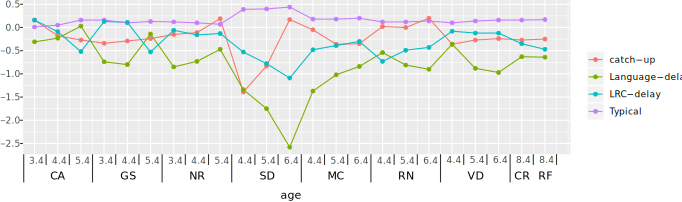
\includegraphics{Lin(2011)}
	\caption{Lin(2011)通过}
	\labfig{Lin(2011)}
\end{figure*}
	
上面的这个实验提到了一种叫混合增长模型的统计技术,我们简要介绍一下它.\reffig{Boscardin(2008)}是Boscardin(2008)的一项研究的结果,这个实验的数据分析就是用的这个模型.最大的图中,可以看到这个数学模型很好地把孩子分成两个亚类型,类型内的孩子比较接近,但是类型间的孩子相差较远;而且这些孩子中,有些孩子斜率相同,起点不同;有些孩子起点相同,斜率不同;也有可能起点不一样斜率也不一样.这就是用到复杂的统计,得到了非常丰富的信息.所以对于数学和统计学习一定要下尽全力,我们不仅要有最精细的实验设计,也要有最复杂的统计分析手段,这样才能做最好的研究,只是大多研究者醒悟的比较晚,若你现在还有心去学数学,那就立马去学吧!

\begin{figure*}
	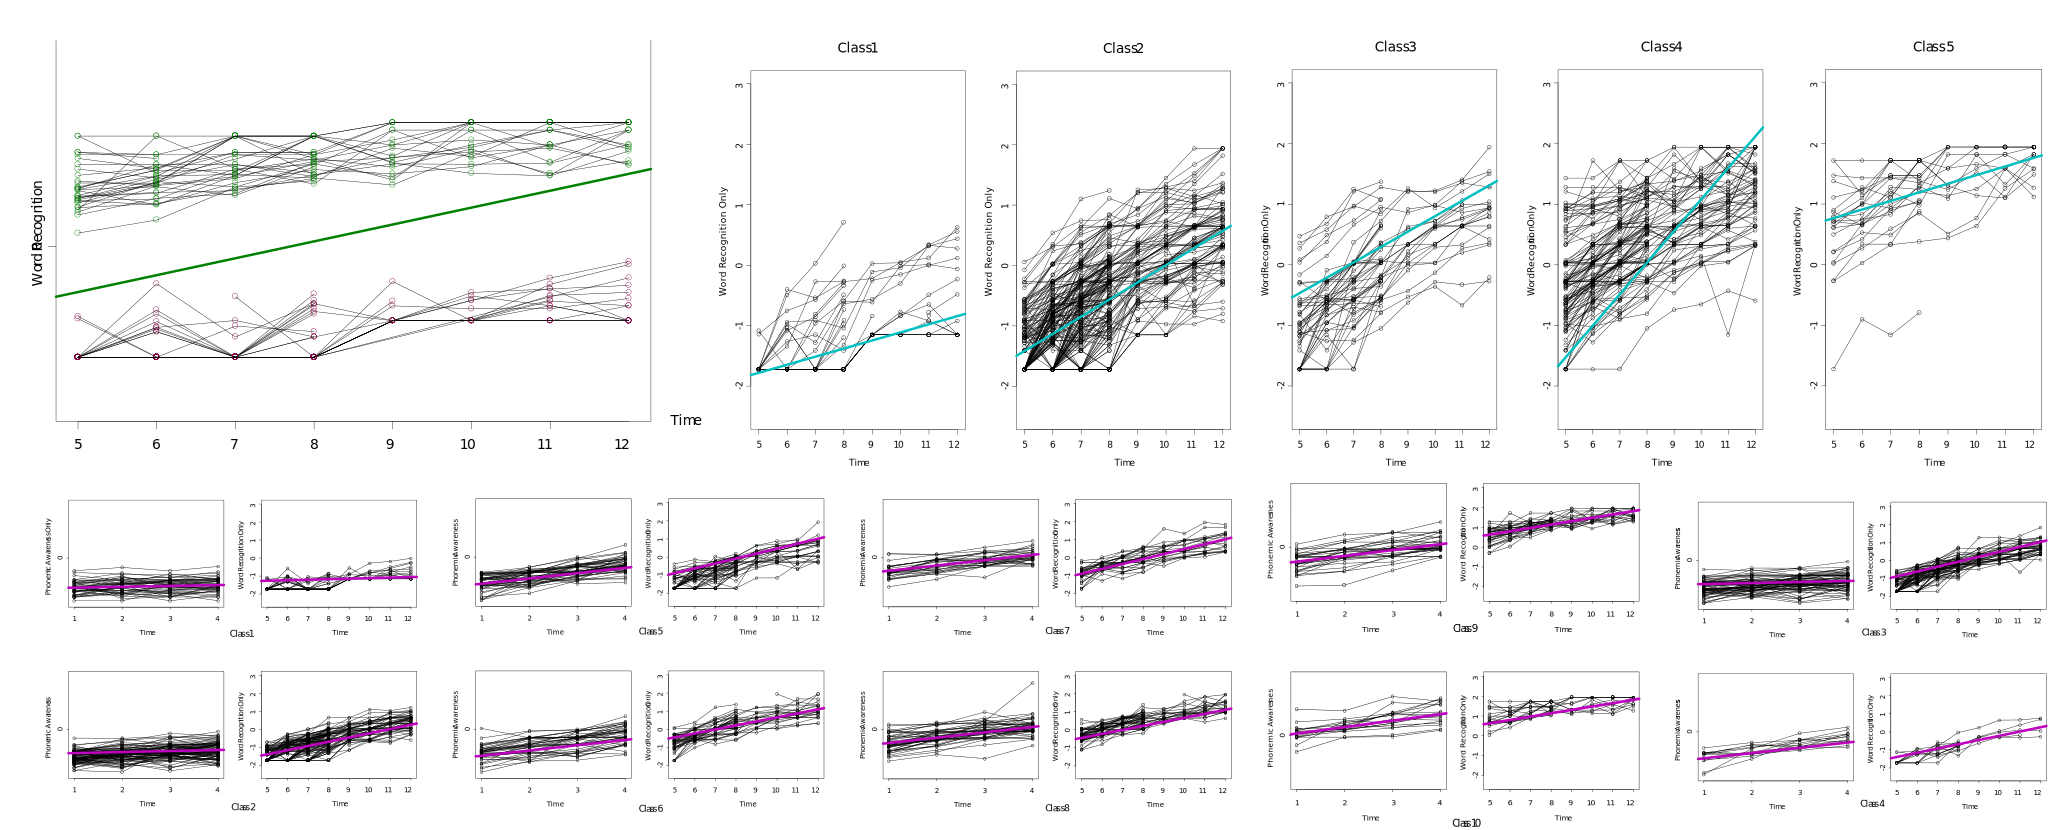
\includegraphics{Boscardin(2008)}
	\caption{Boscardin(2008)}
	\labfig{Boscardin(2008)}
\end{figure*}


前面介绍的部分实验用到了比较新的技术,一方面在工具上,针对于脑研究,像ERP/FMRI/眼动仪都是非常好的研究工具,它们帮助我们从更深层次探讨人脑的奥秘;另一方面,新的统计技术也让研究可以更精确的得出结果,包括已经写入大多课本的多重回归、路径分析、结构方程,也有上面提到的混合增长模型.不论这些手段多么的眼花缭乱,一定要注意,实质仍然是实验设计.比如下面这个实验,虽然仍然是行为学实验,不过实验设计非常有趣,非常漂亮地得到了结论.

\begin{marginfigure}
	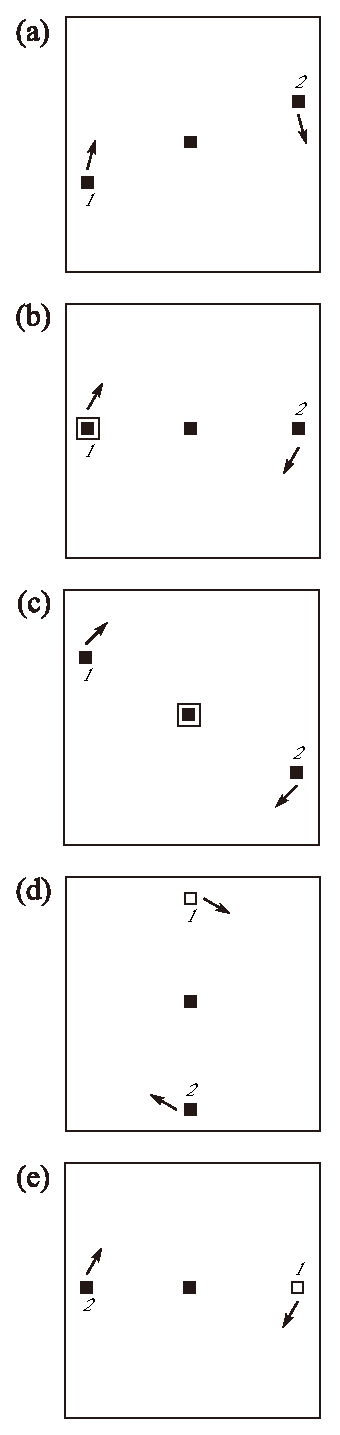
\includegraphics{Tipper(1991)}
	\caption{Tipper(1991)发现了基于物体的注意在返回抑制中相比基于空间的注意更具优势}
	\labfig{Tipper(1991)}
\end{marginfigure}

Tipper(1991)研究了注意中的返回抑制现象(inhibitation of return),所谓返回抑制,大体上是说对于我们注意过空间的某个区域,再次对其注意需要付出更多努力,在行为上的表现就是需要花费更多时间去重新注意.这点在学生看书时表现的很常见,在看完一本书后,我们好像有一种不知道哪里来的抗拒心理让我们不愿意复习.

Tipper想知道的是,我们到底是不愿意再注意注意过的物体,还是不愿意注意注意过的空间位置?若二者都存在抑制效应,哪种注意更占优势呢?\reffig{Tipper(1991)}是他的研究.初始状态a,有三个方块在视野中,方块1、方块2和中间的方块.1和2顺时针旋转到水平时(b),1闪烁,继续旋转到c后中间方块闪烁,然后等到旋转到e,此时1和2的位置和b中正好相反,然后1再次闪烁或者2闪烁,记录这次闪烁到按键间的反应时,发现被试更加难以注意1,说明了基于物体的注意在返回抑制中更有优势.

心理学研究的发展:
实验心理学:拥有严密的实验控制
教育与社会心理学:大样本+统计

复杂实验设计和多元统计的结合

推论统计——从样本推断到总体,不用
1有限的现象:可以观察到全体样本
2可以直接观察:DNA螺旋

统计假说:一种推论形式,可基于不完整的信息检验科学假说的真伪

方差分析的基本思想
对一组数据的描述:集中、离散
X1: 7 5 4 10 4
X2: 10 1 1 15 3
mean:6 6
range:4-10 1-15
var: 26 156

$$
	t=\frac{X_1-X_2}{S_P}
$$

变异是否存在?

施加处理:一致性变化(组内变化没变,组间有变)

随机分配被试来保证实验前被试同质

$$
	F=\frac{MS_{\text{处理效应}}}{MS_{\text{误差效应}}}
$$

下面应该是一个随机误差,所有处理效应要和误差效应相比,